\documentclass[12pt, titlepage]{article}
\usepackage[a4paper,margin=.75in]{geometry}
\usepackage{tgtermes}
\usepackage{amsmath}
\usepackage{setspace}
\usepackage{placeins}
\usepackage{listings}
\usepackage{color}
\usepackage{fancyhdr}
\usepackage{graphicx}
\usepackage[parfill]{parskip}
\usepackage{hyperref}
\hypersetup{
    colorlinks=true,
    linkcolor=blue,
    filecolor=magenta,      
    urlcolor=cyan,
}

\definecolor{dkgreen}{rgb}{0,0.6,0}
\definecolor{gray}{rgb}{0.5,0.5,0.5}
\definecolor{mauve}{rgb}{0.58,0,0.82}

\lstset{frame=none,
  language=Java,
  aboveskip=3mm,
  belowskip=3mm,
  showstringspaces=false,
  columns=flexible,
  basicstyle={\small\ttfamily},
  numbers=none,
  numberstyle=\tiny\color{gray},
  keywordstyle=\color{blue},
  commentstyle=\color{dkgreen},
  stringstyle=\color{mauve},
  breaklines=true,
  breakatwhitespace=true,
  tabsize=3
}

\pagestyle{fancyplain}
\lhead{Sean Connor}
\chead{Project 2 - Analysis}
\rhead{16 July 2018}

\title{Project 2 Analysis}
\author{Sean Connor \\ \\ 605.202 Data Structures \\ \\ 16 July 2018}
\date{}
\singlespacing

\begin{document}

\maketitle

\section {Data Structures}

 The only defined requirements in this project (beside correct calculation of the determinant of a matrix) were that an array be used and that the determinant be calculated using a recursive algorithm. Thus, I did not explicitly create any data structures for this project (i.e. stack, queue, etc). However, recursive methods utilize the ``the stack", which is also known as the call stack, execution stack, program stack, control stack, run-time stack, or machine stack [1].  I am taking 605.204 Computer Organization concurrently with this class, and am learning much more about this topic. With each recursive function call of the det() method, the stack pointer is incremented some amount. The block of memory allocated for a particular instance of the recursive function contains local variables specific to that instance. As the methods conclude, the stack pointer is decremented and the memory is freed up.

To represent a particular matrix, I choose to use a 2-dimensional int[][] array with each dimension being equal to the size of the square matrix i.e. int[size][size]. The int type was used in this case; however, it would be quite simple to use the double type instead if the matrices contained real numbers.

The recursive algorithm functions by breaking each matrix down into smaller matrices, and calling the determinant method on each of those (which in turn may be broken down further). For a square matrix of size n, there will be n submatrices evaluated. This means that each ``block" on the call stack contains information about the matrix and each submatrix, to include an integer representing size and information on the matrix itself (the int[][]). 

Aside from this, no other data structures featured so far in this course were used.

\section{General Strategy}

The recursive algorithm to be used was described in one of the project description files (ALT3.2.6.pdf). It is restated here for convenience.
\begin{equation}
\textrm{det}(a) = \sum_j \textrm{power}(-1, i+j) \times a[i,j] \times \textrm{det}(\textrm{minor}(a[i,j])), \textrm{for any i}
\end{equation}

The recursive method is called det(), and accepts an int[][] as input. Thus, the form of the method is det(int[][] matrix). The first step in implementing this algorithm was defining a base case. The base case was defined to be when the square matrix size was equal to one. At this point, simply return the value. The remainder of the method consists of a series of nested for-loops that iterate through each submatrix, and through each column and row of those submatrices. Each submatrix is stored in an int[][] and passed recursively to the det() method. As mentioned previously, a square matrix of size n will have n submatrices. Each of these submatrices is passed to the det() method. For example, for a square matrix of size three, the det() method will be called a total of ten times. 


\begin{table}[!htbp]
\centering
\begin{tabular}{|c|c|}
\hline
\multicolumn{1}{|l|}{\textbf{size}} & \multicolumn{1}{l|}{\textbf{number of det() calls}} \\ \hline
1                                   & 1                                                   \\ \hline
2                                   & 3                                                   \\ \hline
3                                   & 10                                                  \\ \hline
4                                   & 41                                                  \\ \hline
5                                   & 206                                                 \\ \hline
6                                   & 1237                                                \\ \hline
7                                   & 8660                                                \\ \hline
\end{tabular}
\end{table}

Clearly, the number of recursive calls quickly gets out of hand.

The input was read line by line from a text file using a combination of BufferedReader, InputSteamReader, and FileInputStream. The input text file must be formatted correctly, otherwise the program will produce an error message. Typical errors include empty lines in the text file, improper specification of size, and matrices that are not square. The first line of the input file is read normally. This line specifies the size of the first matrix. After this, the program reads n lines, where n is equal to specified matrix size. After reading each line, the String.split() and Integer.parseInt() methods are employed to split the String into a String[] of numbers, which are then converted to int and placed in an int[][] matrix. Finally, as the reader moves through the input file and calculated the determinants, the matrix information (including determinant) is printed to the console and appended to a StringBuilder object, which is returned and written to specified output file in the main() method using BufferedWriter/OutputStreamWriter/FileOutputStream.

\section{Algorithm Efficiency}

As described previously, this algorithm requires a drastically increasing number of recursive det() calls as the size increases only slightly (see previous table). In fact, it is even worse than (n!)! The efficiency is best characterized as O(n!), which is very bad. To test this, I implemented an execution timer to calculate and print the amount of time it takes to find the determinant of each matrix. I created a test case input file containing diagonal square matrices of size 1 to 11 with the diagonal values ranging from 1 at the upper left corner, and incrementing by 1 to size n at the bottom right corner. 

\[
\begin{bmatrix}
    1 & 0 & 0 & 0 \\
    0 & 2 & 0 & 0 \\
    0 & 0 & 3 & 0 \\
    0 & 0 & 0 & 4
\end{bmatrix}
\]

I evaluated the test case three separate times and recorded time to completion results. These results were plotted in Excel. An exponential curve was created with equation $f(x) \approx 651.103^{1.483x}$ and an R\textsuperscript{2} value of 0.959. See figure below.

As seen in the graphic, the performance of the algorithm aligns well with (n!). Thus, the estimate of O(n!) efficiency is confirmed, at least for values of n up to 11. 

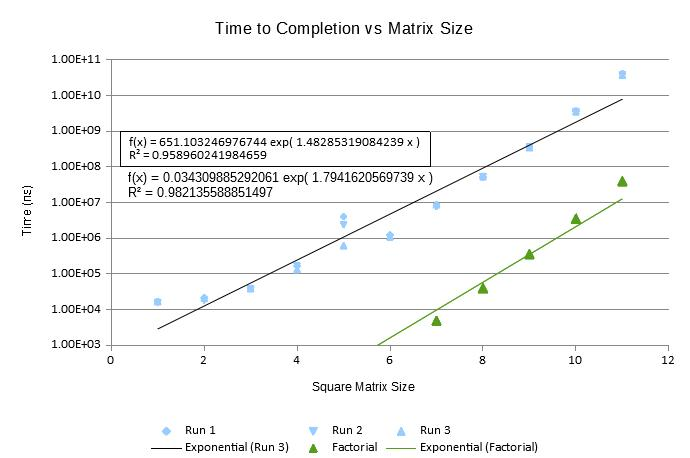
\includegraphics[width=\textwidth]{efficiency}

\section{Iteration}

Any iterative code can be converted to recursive and vice-versa. In this case, the conversion can be achieved by using a series of nested loops. We know that for a matrix of size n, there will be n submatrices to evaluate. Thus, a while loop can be used to iterate through all sizes.
\begin{lstlisting}
/* braingstorming pseudocode for iterative implementation */
while (size > 0) {
	matrix[size]
	while ( i < length ) {
		matrix[i] = ...
	}
	// calculation here to evaluate determinant
}
\end{lstlisting}
A stack could be a good data structure to implement an iterative version. A numerical result is returned beginning at size one evaluation. These numerical results are fed into equations at higher levels/sizes to create numerical results at these levels. Thus, the results from lower levels could be pushed to a stack when calculated, and popped when needed for calculation of determinant at higher levels. It is almost pseudo-recursive, as it implements the same general algorithm without actually calling itself.

\section{Lessons Learned}

This was a great exercise in learning how to utilize implement recursive methods. In addition, it is always good practice learning to handle/process IO for different applications and think creatively to effectively implement methods for this.

One major lesson learned is the importance of algorithm efficiency, and how easy it was in this case for the program execution time to spiral out of control. At around size 12, it was taking my computer more than a minute to calculate. At size 14 it would take hours. Beginning at size 15 it would take days. This served as a great practical example to teach this lesson. Upon some further research, it seems that the most popular algorithm used to find the determinant is Gaussian Elimination. The efficiency of this is O(n\textsuperscript{3}), which is still not ideal but is orders of magnitude faster than O(n!).

I didn't get much practice with different data structures we have learned about, such as stack, queue, and list, but it was a good exercise nonetheless.

\newpage

\section{References}
\begin{enumerate}
	\item ``Call Stack" Wikipedia. \url{https://en.wikipedia.org/wiki/Call_stack}
	\item ``What and where are the stack and heap?" StackOverflow. \url{https://stackoverflow.com/questions/79923/what-and-where-are-the-stack-and-heap}
\end{enumerate}

\end{document}